\subsection{MVP 模式}

MVP模式(Model-View-Presenter pattern)是一种用于分离应用程序的数据模型(Model)、用户界面(View)和业务逻辑(Presenter)的设计模式。

在MVP模式中,Model代表应用程序的数据模型,它负责处理与数据相关的业务逻辑,例如对数据进行验证、查询和修改等。View代表用户界面,它负责显示数据和与用户交互,例如显示表单和按钮等。Presenter负责接收用户的请求,并调用Model和View来完成相应的业务逻辑和显示数据。

与MVC模式相比,MVP模式的一个主要区别在于View与Model之间的交互方式。在MVC模式中,View通常会直接操作Model,而在MVP模式中,View通常不会直接操作Model,而是通过Presenter来操作Model。这样,Presenter就成为了View与Model之间的桥梁,使得View与Model之间的耦合度降到最低。

MVP模式通常用于构建大型的,复杂的应用程序,例如企业应用程序或Web应用程序。它可以帮助开发人员更轻松地处理应用程序的业务逻辑和用户界面,并使应用程序更容易维护和扩展。

\begin{figure}[H]
  \centering
  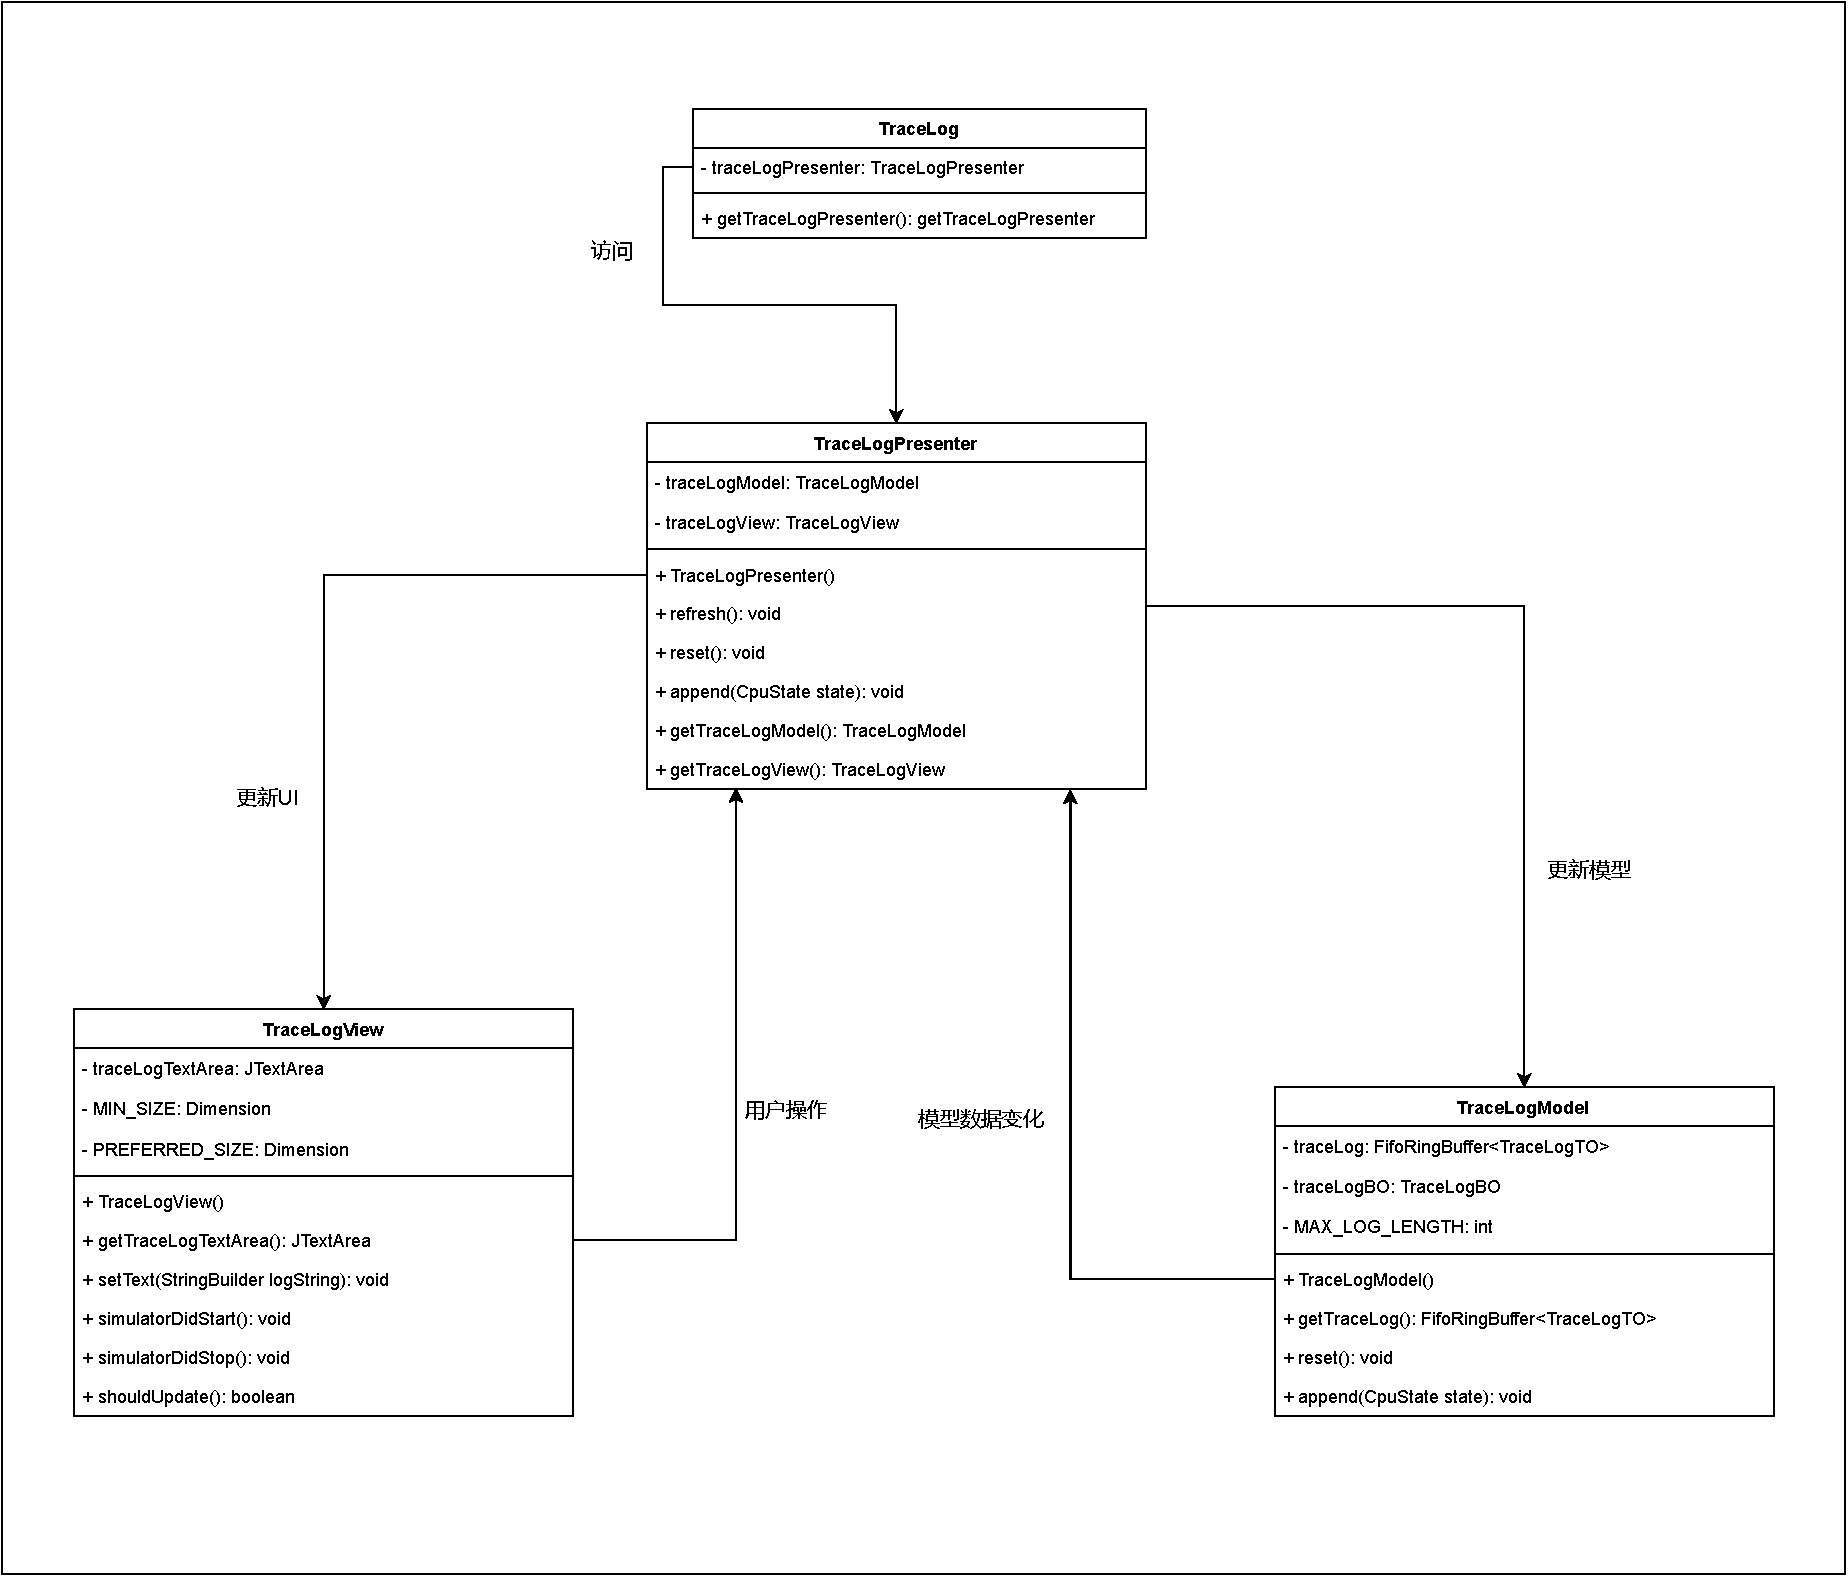
\includegraphics[width=0.9\textwidth]{figures/MVP模式.pdf}
  \caption{MVP 模式在 Slow6502 中的类图}
\end{figure}

对于traceLog的前端功能,通过使用MVP模式,分离了traceLog视图展示的逻辑和traceLog记录与获取的业务逻辑。TraceLogModel类和TraceLogView类是不直接交流的,他们通过TraceLogPresenter沟通,TraceLogPresenter类负责整合TraceLogModel类和TraceLogView类,为系统提供traceLog展示的功能。
